\documentclass[11pt,a4paper]{article}
\usepackage[T1]{fontenc}
\usepackage[utf8]{inputenc}
\usepackage{lmodern,microtype}
\usepackage[margin=.78in]{geometry}
\usepackage{amsmath,amssymb,mathtools,booktabs,tabularx,array,enumitem}
\usepackage{xcolor,mdframed,tikz}
\usetikzlibrary{arrows.meta,positioning}
\usepackage[hidelinks]{hyperref}
\usepackage{fancyhdr}
\setlength{\headheight}{14pt}
\pagestyle{fancy}\fancyhf{}
\lhead{\small Sync HotStuff RR, Part III}\rhead{\small Staking / v4}
\cfoot{\thepage}
\setlength{\parindent}{0pt}\setlength{\parskip}{5pt}
\setlength{\emergencystretch}{2em}
\setlist{nosep,leftmargin=*}
\newcolumntype{Y}{>{\raggedright\arraybackslash}X}
\newcommand{\Hash}{\mathsf H}
\newcommand{\tagg}[1]{\mathsf{#1}}
\newcommand{\cfg}{\mathcal C}
\newcommand{\Ban}{\mathsf{Ban}}
\newcommand{\emin}{e^{\min}}
\newcommand{\cid}{\mathrm{cid}}
\hypersetup{pdftitle={Sync HotStuff RR, Part III: Staking and Authority, v4}}
\begin{document}
\begin{center}
{\Large\bfseries Part III: Staking and Authority}\\[3pt]
{\small Version 4 \quad 24 October 2026}
\end{center}

L1 updates stake in long epochs; regional sessions rotate much faster.
This module turns L1 stake into the authority of every Part~II session:
which region serves, who votes with what weight, and who leads each view.
It also penalizes provable faults and releases stake safely. Part~II sees
only the interface below.

\begin{mdframed}[linewidth=.6pt,innertopmargin=5pt,innerbottommargin=5pt]
\textbf{Core idea.}
\begin{enumerate}[label=\textbf{\arabic*.},itemsep=2pt]
\item \textbf{Four things apart.} Escrow can be slashed; snapshot weight
is frozen; eligibility comes from the branch's status map and the ban
registry; leaders come from a public schedule.
\item \textbf{One L1 read per plan.} A session's plan reads L1 at one
height: the latest activated snapshot and the ban registry there. One
long-epoch snapshot serves many sessions.
\item \textbf{Plan one session ahead.} A regular successor is planned
from its predecessor's initial anchor, but continues after the
predecessor's terminal DATA. A plan grants no signing right.
\item \textbf{Fixed committee, shrinking proposer set.} Members and
weights never change inside a session; only recovery records and later
plans exclude proposers.
\item \textbf{Exit waits for one closure.} A retired position leaves new
snapshots. An effective Force that raises the branch minimum closes every
program that might still use it; funds follow after a holding period.
\end{enumerate}
\end{mdframed}

\paragraph{Interface with Part~II.}\leavevmode\par
\begin{tabularx}{\linewidth}{@{}>{\raggedright\arraybackslash}p{.22\linewidth}Y@{}}\toprule
Part~II calls & Result\\\midrule
$\tagg{Plan}$ & $\Pi=\tagg{Plan}(\mathcal P_\beta,\beta,r,\mathit{cause},E,i_{\rm src})$,
also written $\tagg{AUTH}_{\beta,r,0}$: the session's region or $\bot$,
committee, parameters, source height $\lambda(\Pi)$ and identifier
$\mathrm{id}(\Pi)$ (\S\ref{sec:plan}).\\
$\tagg{AUTH}$, $\tagg{Leader}$ & $\tagg{AUTH}_{\beta,r,g}$ is the proposer set
of generation $g$, and $\tagg{Leader}(\tagg{AUTH}_{\beta,r,g},t)$ the leader
of term $t$ (\S\ref{sec:leaders}).\\
Policy check & Whether a branch update may install a new policy
(\S\ref{sec:policy}).\\\midrule
Part~II reports & Effect on L1\\\midrule
$\tagg{SubmitQuit}$, $\tagg{SubmitOffense}$ & Recovery record; penalty and
ban (\S\ref{sec:account}).\\
$\tagg{ProveForce}$ & Clearance of retired stake (\S\ref{sec:release}).\\\bottomrule
\end{tabularx}

Every function returns a value or \emph{wait}. Missing evidence pauses
the caller; it is never read as zero weight or an empty candidate set.
Part~II binds every regional signature to the session context identifier
\[
 \cid_s=\Hash\bigl(\mathrm{id}(\Pi_s),\Hash(A_s)\bigr),
\]
which this module also uses to attribute recovery records and offenses.

\section{Sessions and anchors}
\label{sec:anchors}
A session $s=(\beta,r)$ is one region's production turn. The branch
version $\beta$ changes on Force; $r$ is a turn index, not a region ID. A
view is $(\beta,r,g,t)$, where $g$ counts recoveries and $t$ leader terms.
For a DATA block $B$, $h(B)$ is its DATA height and $\lambda(B)$ the
finalized L1 height it references. A session continues after its
execution anchor $A_s$ and ends at its terminal DATA $T_s$, at height
$h(A_s)+\mathrm{TB}$.

Its plan uses a separate \emph{selection reference} $E_s$:
\[
 E_s=A_p,\quad A_s=T_p\quad\text{for the regular successor $s$ of $p$};
 \qquad E_s=A_s\quad\text{for the first session of a branch.}
\]
$E_s$ is known once $p$'s boundary is fixed, a full session before $s$
can start; $A_s$ is fixed only when $p$ completes. A Force opens its
first session at the retained tip of Part~II's global prefix $G$; genesis
opens at $A_0$. The source region $i_{\rm src}$ is $p$'s region for a
regular successor, the export session's region for a Force, and $\bot$
at genesis.

\paragraph{Running example.}
A's session $(7,20)$ produces DATA 101--110 after anchor 100. B's regular
successor $(7,21)$ is planned from 100 and continues after 110. Later a
Force activates while $G$ ends at 108; B's new session $(8,21)$ is planned
from 108 and continues after 108. Snapshots $\cfg_7$ and $\cfg_8$ activate
at L1 heights 2000 and 3000, and the Force's policy sets minimum snapshot
8. \S\ref{sec:example} completes the example.

\section{The L1 staking ledger}
\label{sec:ledger}
\subsection{State and parameters}
The ledger is an L1 contract. Its state is public and changes only
through the transitions of this section and of \S\ref{sec:account}.

\begin{tabularx}{\linewidth}{@{}>{\raggedright\arraybackslash}p{.20\linewidth}Y@{}}\toprule
Object & Content\\\midrule
Position $o$ & Permanent ID, region, operator key, withdrawal owner,
escrow $B_o$, lifecycle state, exit index $e_x$ once retired, processed
offenses.\\
Snapshot $\cfg_e$ & Index $e$, cutoff $c_e$, activation height $a_e$,
member positions with frozen integer weights $w_o$ per region, root and
publication height.\\
Ban registry & Operator keys banned from proposing; it only grows.
$\Ban(\ell)$ is its content at finalized L1 height $\ell$.\\
Recovery records & At most one $\tagg{REC}(\cid,g)$ per pair, holding the
ban set it froze (\S\ref{sec:account}).\\
Clearance list & Pairs $(e^\star,t_c)$ with strictly increasing
$e^\star$ (\S\ref{sec:release}).\\\bottomrule
\end{tabularx}

Genesis fixes the chain and algorithm identifiers, the registered regions
$\mathcal L_R$ in a cyclic order, the minimum bond, FIFO amount and count
budgets, entry and exit delays in L1 blocks, the epoch length $M$ and
the notice $N$ with $0<N<M$, the penalty fraction $\rho$, the holding
period $T_{\rm hold}$, the session quota $\mathrm{TB}>0$, the term length
$K$, each region's delay bound $\Delta_i$ and fault fraction
$0\le\varphi_i<1/2$, the snapshot $\cfg_0$, the policy $\mathcal P_0$ with
$\emin_0=0$, and an authenticated DATA anchor $A_0$ with
$\lambda(A_0)\ge a_0$. Escrow and weight are separate: after a penalty,
weight 100 may be backed by only 70 tokens; old certificates still use
100.

\subsection{Lifecycle and snapshots}
\label{sec:lifecycle}
Use one token and whole-position joins and exits. One key belongs to at
most one live position; IDs are never reused. Key or region changes need
a new registration after the old liability is settled.

\begin{center}
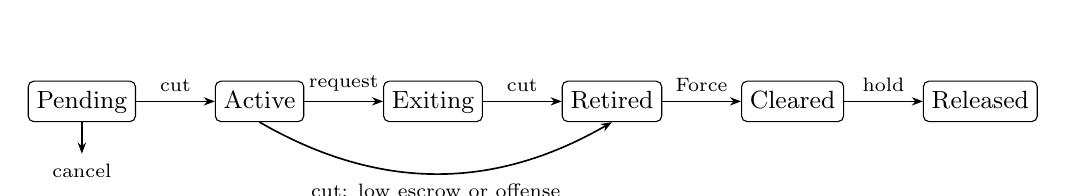
\begin{tikzpicture}[st/.style={draw,rounded corners=2pt,inner sep=3pt,font=\small,
 text height=1.6ex,text depth=.4ex,anchor=base},
 ar/.style={-{Stealth[length=4pt]},semithick},
 lb/.style={font=\scriptsize,midway,above}]
\node[st] (p) {Pending};
\node[st,right=1.0cm of p] (a) {Active};
\node[st,right=1.0cm of a] (x) {Exiting};
\node[st,right=1.0cm of x] (r) {Retired};
\node[st,right=1.0cm of r] (c) {Cleared};
\node[st,right=1.0cm of c] (d) {Released};
\draw[ar] (p)--node[lb]{cut}(a);
\draw[ar] (a)--node[lb]{request}(x);
\draw[ar] (x)--node[lb]{cut}(r);
\draw[ar] (r)--node[lb]{Force}(c);
\draw[ar] (c)--node[lb]{hold}(d);
\draw[ar] (a.south) to[out=-30,in=-150]
  node[font=\scriptsize,below]{cut: low escrow or offense}(r.south);
\draw[ar] (p.south)--++(0,-.4) node[below,font=\scriptsize]{cancel};
\end{tikzpicture}
\end{center}

\begin{tabularx}{\linewidth}{@{}>{\raggedright\arraybackslash}p{.15\linewidth}Y@{}}\toprule
Transition & Rule\\\midrule
Join & The owner deposits at least the minimum bond within the admission
cap, registers region and keys, proves key possession and owner
authorization, and enters the region's inbound FIFO in L1 order.\\
Cancel & Only before any frozen snapshot includes the position; it
leaves the queue and is refunded.\\
Request exit & Only for a position in a frozen snapshot, with no exit
record or pending request. The request is irrevocable and grants no
permission to stop an assigned duty or withdraw funds.\\
Cut & Freezes the next snapshot; see below.\\
Clear, release & \S\ref{sec:release}.\\\bottomrule
\end{tabularx}

\paragraph{Cutting snapshot $e$.}
Snapshot $e$ activates at $a_e=a_0+eM$ and has cutoff $c_e=a_e-N$.
Anyone may cut it at any L1 height at or after $c_e$; the result depends
only on the complete L1 prefix strictly before $c_e$.
\begin{enumerate}[label=\textbf{\arabic*.},itemsep=2pt]
\item Remove every incumbent whose remaining escrow is below the minimum
bond or that has a processed offense, and clear its queue entries.
\item In each region, select the longest mature prefix of each FIFO that
fits its amount and count budgets. Charge joins their locked balances
and voluntary exits their weights in $\cfg_{e-1}$.
\item Include every surviving position, with its remaining escrow as its
integer weight.
\item Give every omitted incumbent $e_x=e$ and an exit record. It appears
in no later snapshot, and its pending exit request is consumed.
\end{enumerate}
A cut made after $a_e$ has the same content, but consumers wait for it.
Inflow and outflow are counted separately, even when their net change is
zero, and no regional stake floor vetoes exit. Penalty losses and
mandatory removals do not use the voluntary budget. A new snapshot
changes only future plans; it never edits a fixed plan. Queue progress
requires continued L1 processing and positive budgets.

\section{Deriving authority}
\label{sec:derive}
Every function in this section is a pure function of authenticated L1
records, genesis constants and its arguments.

\subsection{Branch policy}
\label{sec:policy}
Each branch version $\beta$ has one immutable policy, installed at
genesis or by the branch update that created it (Part~II):
\[
 \mathcal P_\beta=(S_\beta,\mathsf{Ord}_\beta,\emin_\beta).
\]
$S_\beta$ sets every region ON or OFF. $\mathsf{Ord}_\beta$ maps
$(\mathit{cause},r,i_{\rm src})$ to an ordered list of registered regions;
it is drawn from a genesis-fixed family of deterministic rules. The
\emph{default cyclic rule} lists the regions after $i_{\rm src}$ in the
cyclic order and then $i_{\rm src}$ itself, or every region when
$i_{\rm src}=\bot$. Other rules may permute regions per turn, or give a
fixed list for the first session of a branch. $\emin_\beta$ is the
branch's minimum snapshot index. A new policy passes the \emph{policy
check} when its rule belongs to the family, its minimum is at least that
of the previous valid update (or genesis), and $a_{\emin}$ is at most the
L1 height that includes the update.

\subsection{Plans}
\label{sec:plan}
For a target session $(\beta,r)$ opened for $\mathit{cause}$, with
selection reference $E$ and source region $i_{\rm src}$, the plan
$\Pi=\tagg{Plan}(\mathcal P_\beta,\beta,r,\mathit{cause},E,i_{\rm src})$
is computed in four steps.
\begin{enumerate}[label=\textbf{\arabic*.},itemsep=3pt]
\item \textbf{Read height.} Let
\begin{equation}\label{eq:read}
 \ell=\max\{\lambda(E),\,a_{\emin_\beta}\},\qquad
 e=e(\ell)=\max\{e':a_{e'}\le\ell\}.
\end{equation}
Equivalently $e=\max\{\emin_\beta,e(\lambda(E))\}$. Read $\cfg_e$ and
$\Ban_0=\Ban(\ell)$; if either is unavailable, wait.
\item \textbf{Region.} Select the first region $i$ of
$\mathsf{Ord}_\beta(\mathit{cause},r,i_{\rm src})$ with
$S_\beta(i)=\tagg{ON}$ and positive total weight among its members in
$\cfg_e$ that are not banned in $\Ban_0$. If none qualifies,
$\tagg{region}(\Pi)=\bot$ and the boundary stays pending. Missing evidence
is not zero weight.
\item \textbf{Committee.} The committee is every member $o$ of $i$ in
$\cfg_e$, banned or not, with weight $w_o$. Let $W=\sum w_o$ and
$F=\varphi_iW$; certificates need weight greater than $F$. The plan also
carries $\mathrm{TB}$, $K$ and $\Delta_i$.
\item \textbf{Identity and source height.} $\mathrm{id}(\Pi)$ hashes the
chain, $\beta$, $r$, the cause, $h(E)$, $\Hash(E)$, $\lambda(E)$,
$i_{\rm src}$, $e$, the snapshot root, the policy, $i$ and $\Ban_0$. The
source height $\lambda(\Pi)$ is the greatest of $\ell$, the snapshot's
publication height and the L1 height of the policy; the session's first
DATA must reference L1 at or above it.
\end{enumerate}
A regular successor's plan depends only on its predecessor's boundary,
so it is fixed a session ahead; later snapshots, penalties or policies
never edit it. The minimum matters only when it exceeds $e(\lambda(E))$:
after a Force retires old snapshots, an old retained anchor cannot select
them again.

\subsection{Generations and leaders}
\label{sec:leaders}
Generation zero uses the plan: $\tagg{AUTH}_{s,0}=\Pi_s$ and
$\Ban_{s,0}=\Ban_0$. For $g>0$, $\tagg{AUTH}_{s,g}$ is the plan together
with the finalized record $\tagg{REC}(\cid_s,g)$, and $\Ban_{s,g}$ is the
ban set that record froze; until the record is final,
$\tagg{AUTH}_{s,g}$ waits. Let $\mathcal W^g_s$ be the committee members
whose keys are not in $\Ban_{s,g}$, with their original weights. The
leader of view $(\beta,r,g,t)$ is
\begin{equation}\label{eq:leader}
 L_s(g,t)=\tagg{WeightedRand}\bigl(\mathcal W^g_s,\,
 \Hash(\texttt{LEADER},\mathit{chainId},\beta,r,h(E_s),g,t)\bigr).
\end{equation}
$\tagg{WeightedRand}(\mathcal W,z)$ sorts positive integer weights by
position ID, derives an integer $x\in[0,W)$ from $z$ by specified hash
expansion and rejection sampling, and returns the member whose cumulative
interval contains $x$; for weights $(60,30,10)$, $x=73$ selects the
second. An empty set returns $\bot$: wait for a Force, without changing
the voting quorum. The hash takes only coordinates that no producer can
grind; it never takes $\Hash(E_s)$. Different views may select the same
leader, and voting weights stay fixed, including those of banned
proposers.

\subsection{The example, completed}
\label{sec:example}
\begin{tabularx}{\linewidth}{@{}>{\raggedright\arraybackslash}p{.27\linewidth}YY@{}}\toprule
 & Regular B: $(7,21)$ & Force B: $(8,21)$\\\midrule
Reference $E$; $\lambda(E)$ & $A_{(7,20)}=100$; 2500 & retained tip 108; 2600\\
Minimum; read height $\ell$ & $\emin_7\le7$; 2500 & $\emin_8=8$; $\max\{2600,a_8\}=3000$\\
Snapshot & $\cfg_7$ & $\cfg_8$\\
Candidates; status & $(C,B,A)$; C OFF, B ON & $(A,B,C)$; A OFF, B ON\\
Region; seed coordinates & B; $(7,21,100)$ & B; $(8,21,108)$\\
Execution anchor (Part~II) & 110 & 108\\\bottomrule
\end{tabularx}

Both policies here use explicit lists; the default cyclic rule would also
select B. If B's members weigh $(60,30,10)$ and the hash yields $x=73$, the
second member leads $(7,21,0,0)$. B can prepare from the start of
$(7,20)$, but enters only after A's terminal receipt for 110. A newer
snapshot referenced by 110 affects $(7,22)$, not $(7,21)$.

\section{Accountability and release}
\label{sec:account}
\subsection{Offenses and relative verification}
L1 never decides which session really exists: regular handoffs add no L1
transaction, and a session may run ahead of $G$. Every submission is
therefore checked \emph{relative to a claimed context} $C$: a plan and an
anchor hash, with identifier $\cid(C)$. A forged context only produces
records that no real session uses, and an honest key signs only in its
real contexts, so a forged context cannot implicate it.

For one key and one $\cid$, the following signed pairs are offenses. Here
$j$ is the fresh position within a term, and a DRAIN is Part~II's recovery
block carrying no new DATA.

\begin{tabularx}{\linewidth}{@{}>{\raggedright\arraybackslash}p{.24\linewidth}Y@{}}\toprule
Message & Conflict within one $\cid$\\\midrule
PROPOSE & Different admissible DATA/DRAIN proposals at the same $(g,t,j)$,
with Part~II admission and quota evidence.\\
Fresh vote & Different block choices at the same $(g,t,j)$; DATA and DRAIN
share the one-vote rule.\\
NEWVIEW / ANCHOR vote & Different recovery starting blocks (openings)
in one generation, even if one extends the other.\\
FINAL & Different DATA hashes at one height; FINAL has no $g,t$.\\\bottomrule
\end{tabularx}

Timeouts, BLAME, OFF status, forwarding evidence and different QCs for the
same opening are not offenses. A new branch may legitimately reuse a DATA
height.

\paragraph{$\tagg{SubmitOffense}(C,\mathit{ev})$.} Anyone may submit two
signatures by one key, bound to $\cid(C)$, that conflict as above, with the
evidence the table requires, where the key belongs to a position $o$ in
the snapshot of $C$'s plan. A valid proof atomically records the offense,
debits $\min\{\rho w_o,B_o\}$ and bans the key permanently; the next cut
retires $o$. Proofs are deduplicated by position, offense type and
conflict slot, not by serialization. Total debits never exceed escrow;
invalid or incomplete proofs change nothing; no tribunal is needed.

\paragraph{$\tagg{SubmitQuit}(C,g,Q)$.} $Q$ is a complete Part~II quit
proof for generation $g$ of $C$: a BLAME certificate, a leader
equivocation or a NEWVIEW equivocation. It is checked with weights from
$C$'s committee, leaders from $\tagg{Leader}(\tagg{AUTH}_{C,g},\cdot)$, the
terminal QCs that admit its term when $t>0$, and $\tagg{REC}(\cid(C),g)$
when $g>0$. If $Q$ is valid and $\tagg{REC}(\cid(C),g+1)$ does not exist,
the contract first applies any equivocation in $Q$ as an offense, then
creates $\tagg{REC}(\cid(C),g+1)$ with the ban registry as it then stands.
At most one record exists per $(\cid,g)$, and a bare counter cannot
reserve one. Part~II's correct replicas submit every quit proof and wait
for the record's finality before entering $g+1$.

\subsection{Clearance and release}
\label{sec:release}
A retired position may still belong to a running session, possibly ahead
of $G$, or to a planned successor, and L1 cannot enumerate them. Release
therefore waits for a branch-wide closure, which Part~II's control log
provides. Valid updates activate in log order, because their thresholds
strictly increase and at most one activates per Espresso block, and each
executing update increments $\beta$. So update $U_k$ executes exactly when
\begin{equation}\label{eq:eff}
 \beta_{\rm target}(U_k)=\#\{\,j<k:\ U_j\text{ executes}\,\},
\end{equation}
counted from the genesis control prefix. Call this $\tagg{Eff}(U_k)$; the
control contract computes it when $U_k$ is submitted.

\paragraph{$\tagg{ProveForce}(U,J)$.} Anyone may submit a valid update $U$
with $\tagg{Eff}(U)$ and a finalized Espresso header $J$ whose timestamp
is at least $\theta_a(U)$, verified through Espresso's L1 light client.
If $\emin(U)$ exceeds the last clearance index, L1 appends
$(\emin(U),t_c)$, where $t_c$ is the real time it accepts the proof.
Neither $G$ nor any DATA is read.

This closure suffices for every position with $e_x\le\emin(U)$. Its exit
record precedes $U$, since
$c_{e_x}<a_{e_x}\le a_{\emin(U)}$, which is at most the L1 height of $U$.
At activation, Part~II terminates every program of the closed branch,
including sessions ahead of $G$ and planned successors. Every later plan
uses a snapshot of index at least $\emin(U)$, because minima never
decrease, and no such snapshot contains the position.

\paragraph{$\tagg{Release}(o)$.} The owner may withdraw the remaining
escrow once, strictly after $t_c+T_{\rm hold}$ for the first clearance pair
with $e^\star\ge e_x(o)$, and after applying the valid offense proofs
accepted by then. Part~II bounds closure delivery by $T_E$ and delivery of
available complete results by $T_{\rm pub}+T_E$. Let $T_{\rm ev}$ cover the
additional investigation, collection and submission of evidence,
including from discarded sessions, and let valid slash transactions
finalize within $T_{\rm L1}^{\rm stake}$ of submission. Choose
\begin{equation}\label{eq:hold}
 T_{\rm hold}\ge 2T_E+T_{\rm pub}+T_{\rm ev}+T_{\rm L1}^{\rm stake}
 +\varepsilon_{\rm clock}.
\end{equation}
The first $T_E$ lets nodes learn the closure; $T_{\rm pub}+T_E$ covers
their remaining result delivery. Since $t_c$ is no earlier than the
activation, this measure is conservative. The deployed L1 timelock and
clock margin must prevent expiry before this real interval. Before
release, the operator's data must already be retained by remaining
members or durably transferred under Part~II; afterwards it has no duty.
A finite window cannot catch evidence hidden forever.

\section{Guarantees and costs}
\label{sec:guarantees}
\begin{tabularx}{\linewidth}{@{}>{\raggedright\arraybackslash}p{.24\linewidth}Y@{}}\toprule
Guarantee to Part~II & Statement\\\midrule
G1 Determinism & The same authenticated records give every verifier the
same plan, authority and leader; missing evidence gives wait.\\
G2 Immutability & A plan never changes once computable; each
$(\cid,g)$ has at most one recovery record.\\
G3 Lookahead & A regular successor's plan is fixed with its predecessor's
boundary; regular handoffs and term changes need no L1 transaction.\\
G4 Fixed committee & Members and weights are the same in every generation
and term of a session; penalties change escrow only.\\
G5 Threshold & Weights are positive integers and $F<W/2$.\\
G6 Monotone exclusion & Bans only grow, $\Ban_{s,g}\subseteq\Ban_{s,g+1}$,
and no leader is in $\Ban_{s,g}$.\\
G7 Exit isolation & If $e_x(o)\le\emin_\beta$, then $o$ is in no committee
of branch $\beta$ or of any later branch.\\\bottomrule
\end{tabularx}

In return, Part~II passes the selection reference of \S\ref{sec:anchors},
installs one immutable policy per branch, binds every signature to
$\cid$, submits every quit proof, closes every program of a branch at its
effective Force, and meets its delivery bounds $T_E$, $T_{\rm pub}$ and
$T_{\rm L1}$. With these, Part~I's finalized-authority premise holds:
generation zero is available in advance, and each later generation within
$T_{\rm L1}$ of its quit proof's submission. Part~I's exclusion premise
holds once offense evidence is submitted, because the next recovery record
or plan bans the key. Schedule fairness remains a premise, not a theorem
of this module.

\paragraph{Accepted costs and limits.}
\begin{itemize}[itemsep=3pt]
\item The schedule is public and predictable. Height hashing proves
neither unpredictability nor resistance to identity selection. The
producer of a selection reference chooses its L1 reference within the
allowed range and so, near an epoch boundary, may choose between two
snapshots.
\item Adoption lags by about one session: new stake and new bans reach
generation zero only through later plans. Recovery still waits for L1.
Penalties do not reweight a running committee, and each committee's
frozen-weight fault bound remains a Part~II premise.
\item Release needs an effective Force with a raised minimum and external
services; it has no unconditional time bound, and the Force may discard
production beyond $G$.
\item A proven offender leaves at the next cut, even with enough escrow.
Whole-position exits keep this version small; partial exits, delegation
and parameter changes need explicit extensions.
\end{itemize}

\paragraph{References.}
Part~II v4.7: authority interface, session contexts, full-view leaders,
FINAL, Force-close and service bounds.
Part~I: recovery authority, proposer exclusion and conditional progress.
For queue and lifecycle patterns, see Ethereum's
\href{https://ethereum.github.io/consensus-specs/specs/fulu/beacon-chain/}{Fulu pending deposits}
and \href{https://ethereum.github.io/consensus-specs/specs/electra/beacon-chain/}{Electra exit and slashing rules}.
Their withdrawal constants are not imported here.
\end{document}
